\documentclass{beamer}
\usetheme{Rochester}
% \usecolortheme{seagull}
\usecolortheme{whale}
%\setbeamertemplate{footline} % To remove the footer line in all slides uncomment this line
\setbeamertemplate{footline}[page number] % To replace the footer line in all slides with a simple slide count uncomment this line
\setbeamertemplate{navigation symbols}{} % To remove the navigation symbols from the bottom of all slides uncomment this line
\usepackage{graphicx, booktabs} 

\title{Multi-Agents and Agent Systems}
\subtitle{Flying Saucers Bakery}
\author{Md Zahidussaman, Arun Prabhu, Dharmin Bakaraniya}
\institute{H-BRS}
\date{\today}
\begin{document}

\begin{frame}
    \titlepage{}
\end{frame}

\begin{frame}{Overview}
    \tableofcontents
\end{frame}

\section{Baking stage}%
\label{sec:baking_stage}
\begin{frame}
    \frametitle{\huge{Baking Stage}}
    \begin{columns}[t]
        \column{.45\textwidth}
        \begin{figure}[H]
            \centering
            % \caption{Baking stage component diagram\label{fig:baking_component_diagram} }
            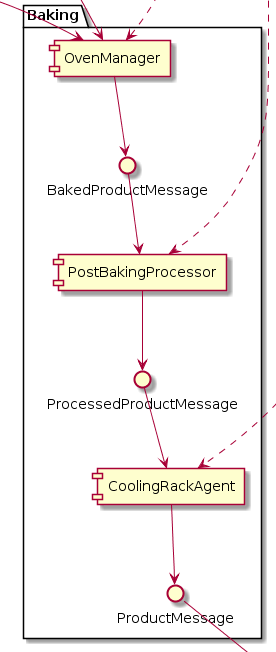
\includegraphics[width=0.6\linewidth]{baking_component_diagram.png}
        \end{figure}
        \column{.5\textwidth}
            \textbf{Agents}
            \begin{itemize}
                \item OvenManager
                \item PostBakingProcessor
                \item CoolingRackAgent
            \end{itemize}
    \end{columns}
\end{frame}
\begin{frame}
    \frametitle{\huge{OvenManager}}
    \begin{columns}[t]
        \column{.45\textwidth}
        \begin{figure}[H]
            \centering
            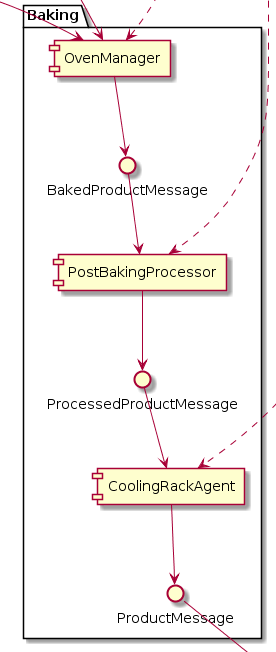
\includegraphics[width=0.6\linewidth]{baking_component_diagram.png}
        \end{figure}
        \column{.5\textwidth}
            \textbf{Agents}
            \begin{itemize}
                \item OvenManager
                \item PostBakingProcessor
                \item CoolingRackAgent
            \end{itemize}
    \end{columns}
\end{frame}
\begin{frame}
    \frametitle{\huge{PostBakingProcessor}}
    \begin{columns}[t]
        \column{.45\textwidth}
        \begin{figure}[H]
            \centering
            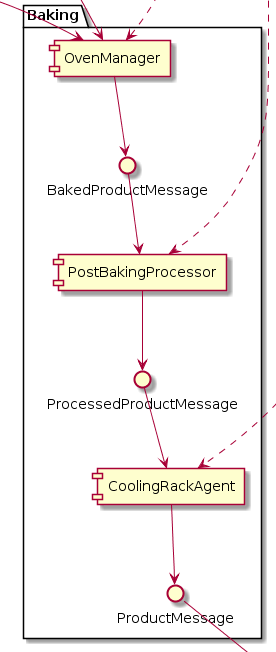
\includegraphics[width=0.6\linewidth]{baking_component_diagram.png}
        \end{figure}
        \column{.5\textwidth}
            \textbf{Agents}
            \begin{itemize}
                \item OvenManager
                \item PostBakingProcessor
                \item CoolingRackAgent
            \end{itemize}
    \end{columns}
\end{frame}
\begin{frame}
    \frametitle{\huge{CoolingRackAgent}}
    \begin{columns}[t]
        \column{.45\textwidth}
        \begin{figure}[H]
            \centering
            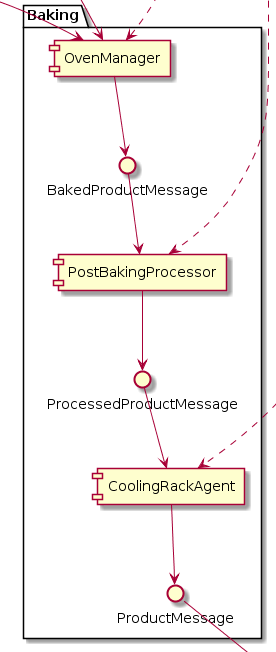
\includegraphics[width=0.6\linewidth]{baking_component_diagram.png}
        \end{figure}
        \column{.5\textwidth}
            \textbf{Agents}
            \begin{itemize}
                \item OvenManager
                \item PostBakingProcessor
                \item CoolingRackAgent
            \end{itemize}
    \end{columns}
\end{frame}

\section{Packaging stage}%
\label{sec:packaging_stage}
\begin{frame}
    \frametitle{\huge{Packaging Stage}}
    \begin{columns}[t]
        \column{.45\textwidth}
        \begin{figure}[H]
            \centering
            % \caption{Baking stage component diagram\label{fig:baking_component_diagram} }
            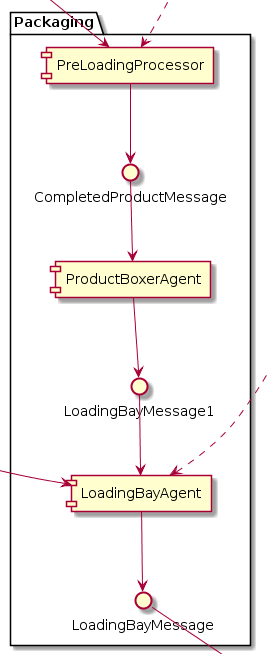
\includegraphics[width=0.55\linewidth]{packaging_component_diagram.png}
        \end{figure}
        \column{.5\textwidth}
            \textbf{Agents}
            \begin{itemize}
                \item PreLoadingProcessor
                \item ProductBoxerAgent
                \item LoadingBayAgent
            \end{itemize}
    \end{columns}
\end{frame}
\begin{frame}
    \frametitle{\huge{PreLoadingProcessor}}
    \begin{columns}[t]
        \column{.45\textwidth}
        \begin{figure}[H]
            \centering
            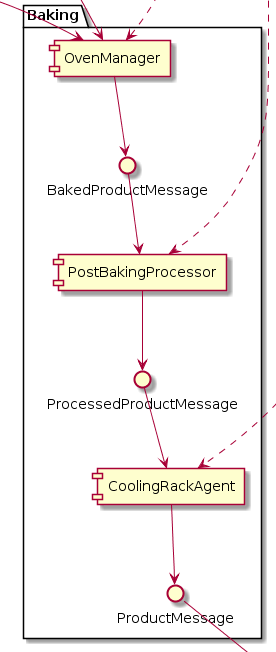
\includegraphics[width=0.6\linewidth]{baking_component_diagram.png}
        \end{figure}
        \column{.5\textwidth}
            \textbf{Agents}
            \begin{itemize}
                \item OvenManager
                \item PostBakingProcessor
                \item CoolingRackAgent
            \end{itemize}
    \end{columns}
\end{frame}
\begin{frame}
    \frametitle{\huge{ProductBoxerAgent}}
    \begin{columns}[t]
        \column{.45\textwidth}
        \begin{figure}[H]
            \centering
            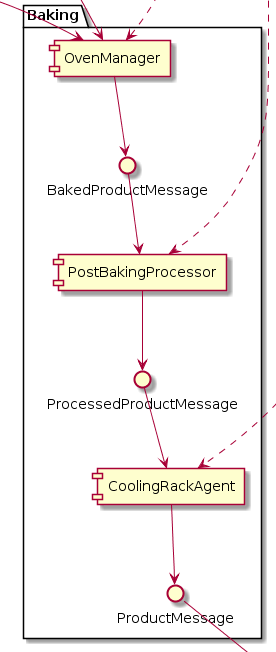
\includegraphics[width=0.6\linewidth]{baking_component_diagram.png}
        \end{figure}
        \column{.5\textwidth}
            \textbf{Agents}
            \begin{itemize}
                \item OvenManager
                \item PostBakingProcessor
                \item CoolingRackAgent
            \end{itemize}
    \end{columns}
\end{frame}

\section{Common agents}%
\label{sec:common_agents}
\begin{frame}
    \frametitle{\huge{Common agents}}
    \begin{columns}[t]
        \column{.45\textwidth}
        \begin{figure}[H]
            \centering
            % \caption{Baking stage component diagram\label{fig:baking_component_diagram} }
            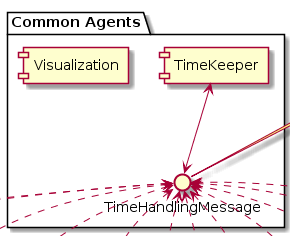
\includegraphics[width=0.75\linewidth]{common_component_diagram.png}
        \end{figure}
        \column{.5\textwidth}
            \textbf{Agents}
            \begin{itemize}
                \item TimeKeeper
                \item BaseAgent
                \item VisualisationAgent (Order board)
            \end{itemize}
    \end{columns}
\end{frame}
\begin{frame}
    \frametitle{\huge{TimeKeeper}}
    \begin{columns}[t]
        \column{.45\textwidth}
        \begin{figure}[H]
            \centering
            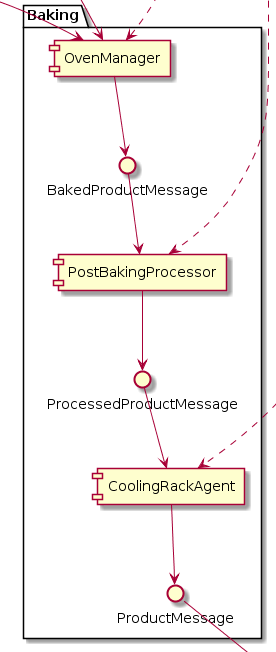
\includegraphics[width=0.6\linewidth]{baking_component_diagram.png}
        \end{figure}
        \column{.5\textwidth}
            \textbf{Agents}
            \begin{itemize}
                \item OvenManager
                \item PostBakingProcessor
                \item CoolingRackAgent
            \end{itemize}
    \end{columns}
\end{frame}
\begin{frame}
    \frametitle{\huge{BaseAgent}}
    \begin{columns}[t]
        \column{.45\textwidth}
        \begin{figure}[H]
            \centering
            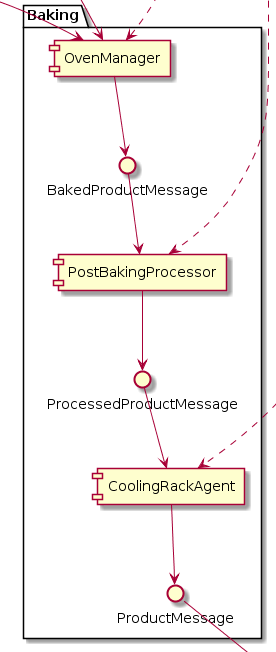
\includegraphics[width=0.6\linewidth]{baking_component_diagram.png}
        \end{figure}
        \column{.5\textwidth}
            \textbf{Agents}
            \begin{itemize}
                \item OvenManager
                \item PostBakingProcessor
                \item CoolingRackAgent
            \end{itemize}
    \end{columns}
\end{frame}
\begin{frame}
    \frametitle{\huge{VisualisationAgent}}
    \begin{columns}[t]
        \column{.45\textwidth}
        \begin{figure}[H]
            \centering
            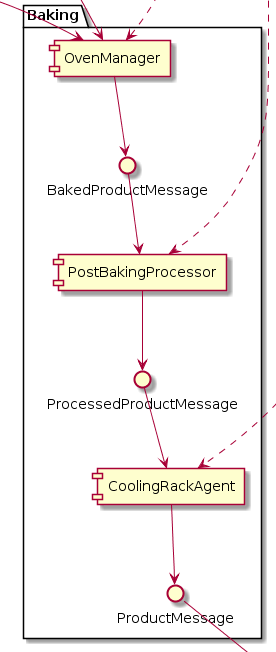
\includegraphics[width=0.6\linewidth]{baking_component_diagram.png}
        \end{figure}
        \column{.5\textwidth}
            \textbf{Agents}
            \begin{itemize}
                \item OvenManager
                \item PostBakingProcessor
                \item CoolingRackAgent
            \end{itemize}
    \end{columns}
\end{frame}

\begin{frame}
    \Huge{\centerline{Thank you}}
    \Huge{\centerline{Demo}}
\end{frame}


%\begin{frame}
%    \frametitle{\huge{Blocks of Highlighted Text}}
%    \begin{block}{Block 1}
%        Lorem ipsum dolor sit amet, consectetur adipiscing elit. Integer lectus nisl, ultricies in feugiat rutrum, porttitor sit amet augue. Aliquam ut tortor mauris. Sed volutpat ante purus, quis accumsan dolor.
%    \end{block}
%\end{frame}
%
%\begin{frame}
%    \frametitle{\huge{Multiple Columns}}
%    \begin{columns}[t]
%        \column{.45\textwidth}
%        \textbf{Heading}
%        \begin{enumerate}
%            \item Statement
%        \end{enumerate}
%        \column{.5\textwidth}
%        Lorem ipsum dolor sit amet, consectetur adipiscing elit. Integer lectus nisl, ultricies in feugiat rutrum, porttitor sit amet augue. Aliquam ut tortor mauris. Sed volutpat ante purus, quis accumsan dolor.
%    \end{columns}
%\end{frame}
%
%\begin{frame}
%    \frametitle{\huge{References}}
%        \footnotesize{
%        \begin{thebibliography}{1}
%            \bibitem[Smith, 2012]{p1} John Smith (2012) Some pub, some date
%        \end{thebibliography}
%}
%\end{frame}
%
%\begin{frame}
%    \Huge{\centerline{Thank you}}
%\end{frame}
\end{document} 
